\documentclass[../main.tex]{subfile}

\begin{document}

\topictitle{Integration}

Integrating polar curves is very finicky. To find the simple area of a polar curve between the angles $\alpha$ and $\beta$, use $$\boxed{\frac{1}{2} \int\limits_{\alpha}^{\beta} r^2 \diffd\theta}$$

\begin{figure}[H]
\hspace{0.02\linewidth}
\begin{minipage}{0.35\linewidth}
	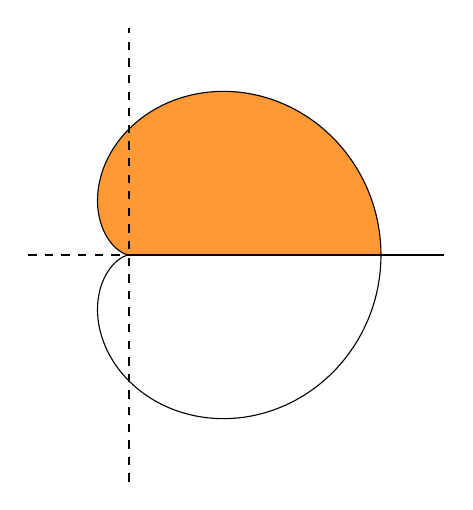
\begin{tikzpicture}[scale=1.6]
		\fill[orange, opacity=0.8, domain=0:180, smooth, samples=250]
			plot (\x:{1 + cos(\x)});

		\draw[dashed] (-0.8,0) -- (0,0);
		\draw (0,0) -- (2.5,0);
		\draw[dashed] (0,-1.8) -- (0,1.8);

		\draw[domain=0:360, smooth, samples=500] plot (\x:{1 + cos(\x)});
	\end{tikzpicture}
\end{minipage}\hfill
\begin{minipage}{0.55\linewidth}
	\setlength{\parskip}{1em}
	This works fine for simple curves like this cardioid, which has shaded area given by $\displaystyle \frac{1}{2} \int_0^\pi (1 + \cos\theta)^2 \diffd\theta$.

	To find the area of the whole thing, we could integrate from $0$ to $2\pi$, or we could integrate from $0$ to $\pi$ again and double the area. These are equivalent by symmetry.
\end{minipage}
\hspace{0.02\linewidth}
\end{figure}

Exams will often ask for more complicated areas, like the one shaded in orange on the left here. To find an area like that, we can decompose the diagram like so.

Draw a line from the origin to separate the region and find the angle $\theta$ that this line makes with the horizontal. Then in this example, the area is $\displaystyle {\color{purple!80}\frac{1}{2}\int_0^\frac{\pi}{3} f(\theta)^2 \diffd\theta} + {\color{blue!80}\frac{1}{2}\int_\frac{\pi}{3}^\frac{\pi}{2} g(\theta)^2 \diffd\theta}$.

\begin{figure}[H]
\hspace{0.02\linewidth}
\begin{minipage}{0.44\linewidth}
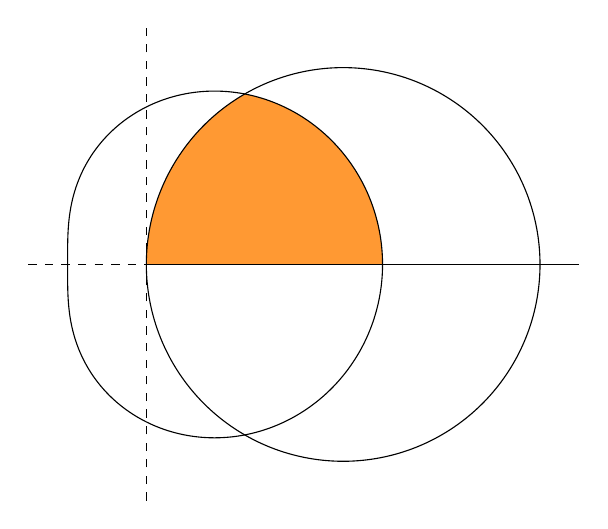
\begin{tikzpicture}
	\coordinate (A) at (60:5/2);

	\fill[orange, opacity=0.8]
		plot[domain=0:60, smooth, samples=250] (\x:{2 + cos(\x)})
		-- plot[domain=60:90, smooth, samples=250] (\x:{5 * cos(\x)})
		-- cycle;

	\draw[dashed] (-1.5,0) -- (0,0);
	\draw (0,0) -- (5.5,0);
	\draw[dashed] (0,-3) -- (0,3);

	\draw[domain=0:360, smooth, samples=500] plot (\x:{(2 + cos(\x))});
	\draw[domain=0:360, smooth, samples=500] plot (\x:{(5 * cos(\x))});
\end{tikzpicture}
\end{minipage}\hfill
\begin{minipage}{0.44\linewidth}
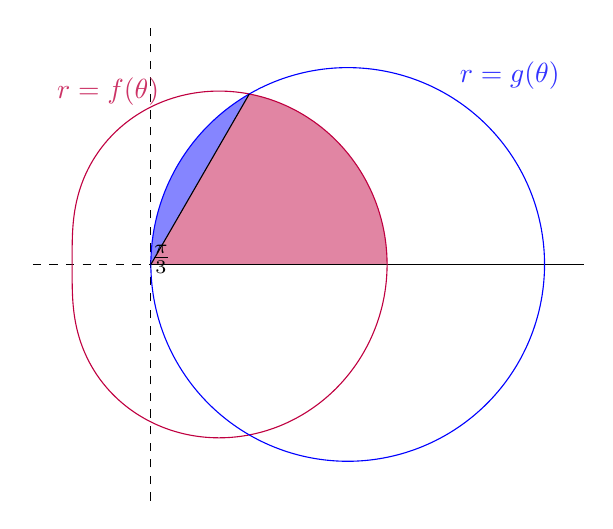
\begin{tikzpicture}
	\coordinate (A) at (60:5/2);
	\coordinate (O) at (0,0);

	\fill[purple!60, opacity=0.8, domain=0:60, smooth, samples=250]
		plot (\x:{2 + cos(\x)}) -- (O) -- cycle;
	\fill[blue!60, opacity=0.8, domain=60:90, smooth, samples=250]
		plot (\x:{5 * cos(\x)}) -- cycle;

	\draw[dashed] (-1.5,0) -- (0,0);
	\draw (0,0) -- (5.5,0);
	\draw[dashed] (0,-3) -- (0,3);

	\draw[purple, domain=0:360, smooth, samples=500] plot (\x:{(2 + cos(\x))});
	\draw[blue, domain=0:360, smooth, samples=500] plot (\x:{(5 * cos(\x))});

	\draw (O) -- (A);
	\coordinate (B) at (1,0);
	\tkzMarkAngle[size=0.8](B,O,A);
	\tkzLabelAngle[pos=0.5](B,O,A){$\frac{\pi}{3}$};

	\node[purple!80] (f) at (-0.8, 2.2) {$r = f(\theta)$};
	\node[blue!80] (g) at (4.3, 2.4) {$r = g(\theta)$};
\end{tikzpicture}
\hspace{0.02\linewidth}
\end{minipage}
\end{figure}

The hardest part of polar integration for me is making sure that the angles are tight. You would think that integrating through a region that seems to have no curve would yield no extra area and not change the answer. However, because we square the equation before putting it in the integral, any negative values of $r$ become positive, so they get counted in the integral. This results in extra area that we don't want, which obviously makes the answer wrong.

The solution to this problem is to \underline{be \textbf{very careful} with the angle bounds of the integrals}.

\end{document}
